\section*{Моделирование СМО}
\addcontentsline{toc}{section}{Моделирование СМО}
\subsection*{Модель СМО в AnyLogic}
\addcontentsline{toc}{subsection}{Модель СМО в AnyLogic}

\textbf{Задание:}\\
Создать и проанализировать модель системы массового обслуживания на примере банка в AnyLogic.\\

\textbf{Решение:}\\
Создадим простейшую модель обслуживания клиентов банка. Обслуживающими блоками будут банкомат и кассиры. Для создания модели будем использовать Библиотеку моделирования процессов. Каждый блок будет задавать определённый элемент СМО.\\

Базовая схема СМО представлена на рисунке \ref{fig:anylogic_bank1}. Данная схема моделирует простейшую СМО, состоящую из источника заявок, очереди, обслуживающего блока. и блока финального уничтожения агентов.
\begin{figure}[h]
	\centering 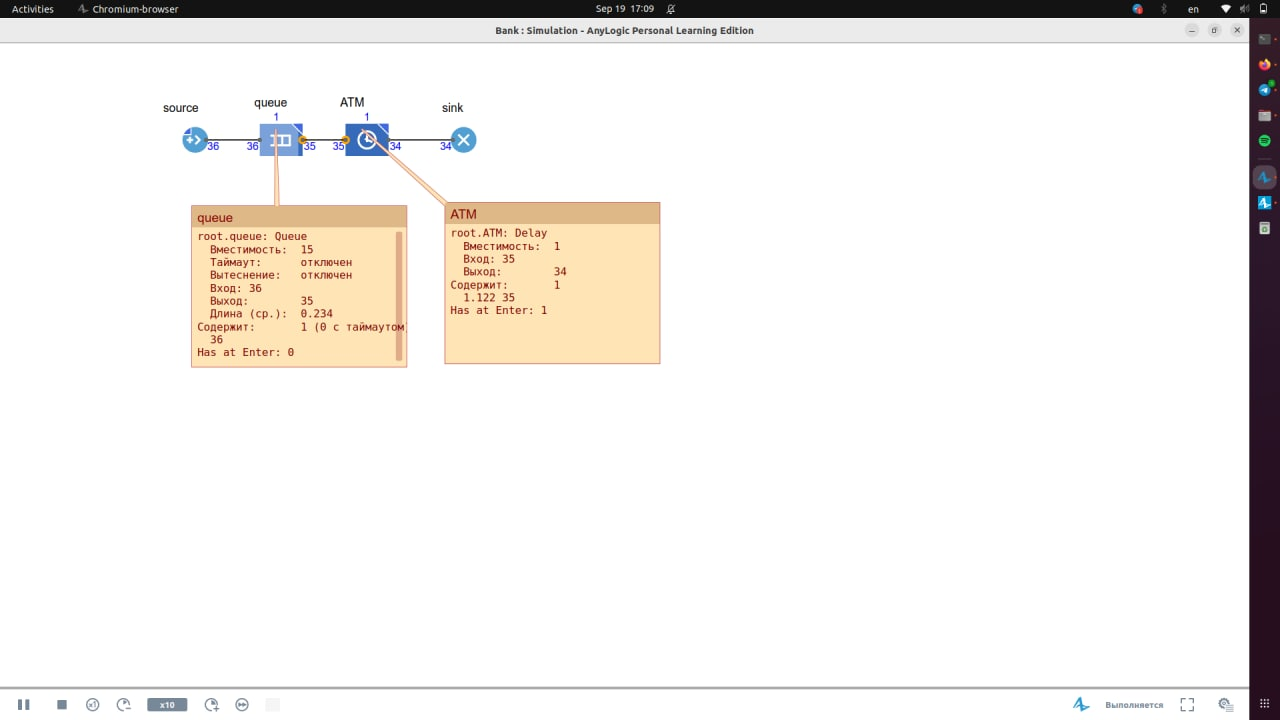
\includegraphics[scale=0.5]{anylogic_bank1}
	\caption{Схема модели простейшей СМО}
	\label{fig:anylogic_bank1}
\end{figure}

В модели задействованы следующие блоки:
\begin{enumerate}[topsep=0pt,itemsep=-1ex,partopsep=1ex,parsep=1ex]
	\item \textit{Source} генерирует агентов определенного типа. Обычно он используется в качестве начальной точки диаграммы процесса, формализующей поток агентов. В нашем примере агентами будут посетители банка, а объект Source будет моделировать их приход в банковское отделение.
	\item \textit{Queue} моделирует очередь агентов, ожидающих приема объектами, следующими за данным в диаграмме процесса. В нашем случае он будет моделировать очередь клиентов, ждущих освобождения банкомата.
	\item Объект \textit{Delay} задерживает агентов на заданный период времени, представляя в модели банкомат, у которого посетитель банковского отделения тратит некоторое время для проведения необходимой ему операции.
	\item Объект \textit{Sink} утилизирует заявки, обработанные системой. Обычно он используется в качестве конечной точки потока агентов (и диаграммы процесса соответственно).\\
\end{enumerate}

Далее в модель была добавлена 2D и 3D анимация того, как агенты (люди) заходят в модель и ожидают в очереди к банкомату. Получившаяся модель представлена на рисунке \ref{fig:anylogic_bank2}.\\
\begin{figure}[h]
	\centering 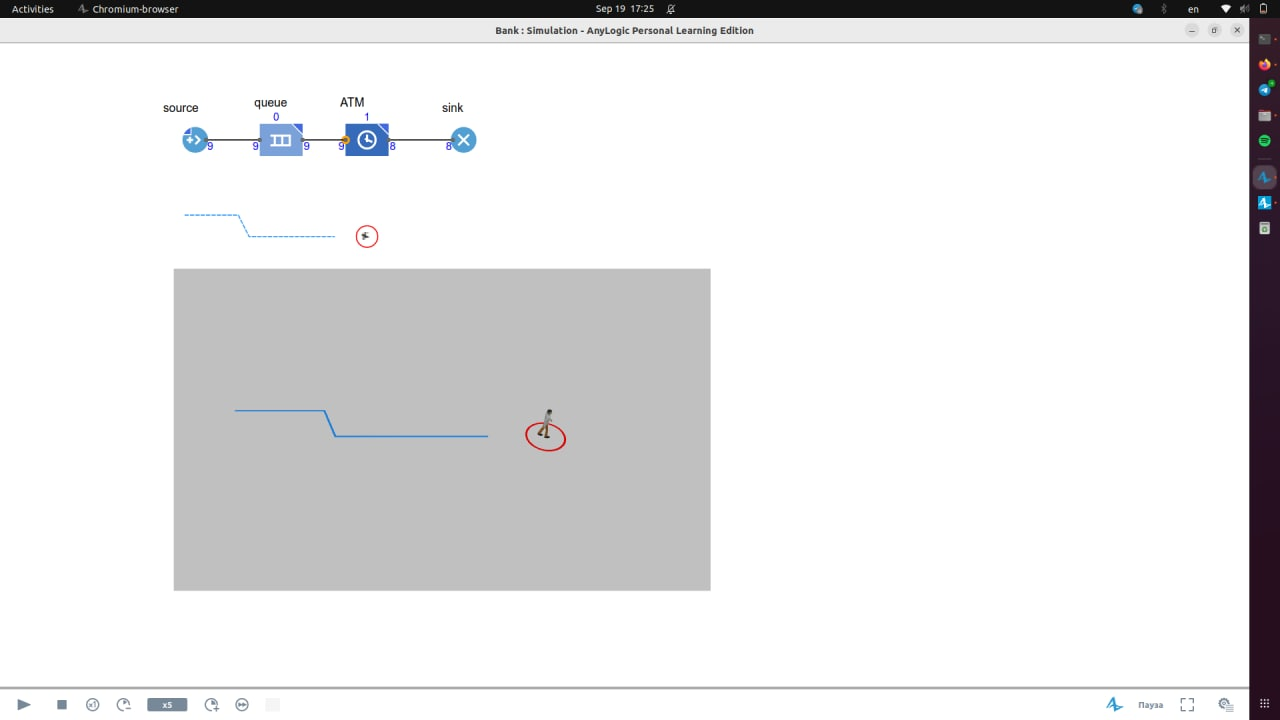
\includegraphics[scale=0.5]{anylogic_bank2}
	\caption{Анимация модели в среде AnyLogic}
	\label{fig:anylogic_bank2}
\end{figure}

\newpage

Далее модель была усложнена. Были добавлены служащие -- банковские кассиры. Можно промоделировать кассиров, как и банкомат, с помощью объекта \textit{Delay}. Но удобнее моделировать кассиров с помощью ресурсов. Объект \textit{Service} захватывает для агента заданное количество ресурсов, задерживает агента, а затем освобождает захваченные им ресурсы.\\

Следующим этапом был добавлен выбор клиентов, то есть агенты могут пойти либо к банкомату, либо к банковским кассирам. Данная логика была реализована с помощью блока \textit{SelectOutput}, он является блоком принятия решения. В зависимости от заданного условия, агент, поступивший в объект, будет отправляться на один из двух выходных портов.\\

Также был добавлен блок \textit{ResourcePool}, который необходим для хранения ресурсов модели. В данном случае в качестве ресурсов будут выступать кассиры.\\


Также в блоке \textit{Source} установим интенсивность прибытья клиентов 0.3 в минуту, т.е. каждые 10 минут будет приходить по 3 человека. В свойствах блока \textit{Queue} установим вместимость 15, то есть в очереди может находиться не более 15 человек. В свойствах блока \textit{Delay} время задержки зададим как $triangular(0.8, 1.5, 3.5)$, т.е. в виде треугольного распределения с минимальным временем обслуживания 0.8 секунд, среднем временем обслуживания -- 1.5 секунды и максимальным -- 3.5 секунд. В блоке \textit{Service} зададим вместимость очереди 20 человек, а время задержки как $triangular(2.5, 6, 11)$. Количество ресурсов, т.е. количество кассиров, установим равным 4.

Теперь модель будет выглядеть следующим образом, как показана на рисунке \ref{fig:anylogic_bank3}.\\
\begin{figure}[h]
	\centering 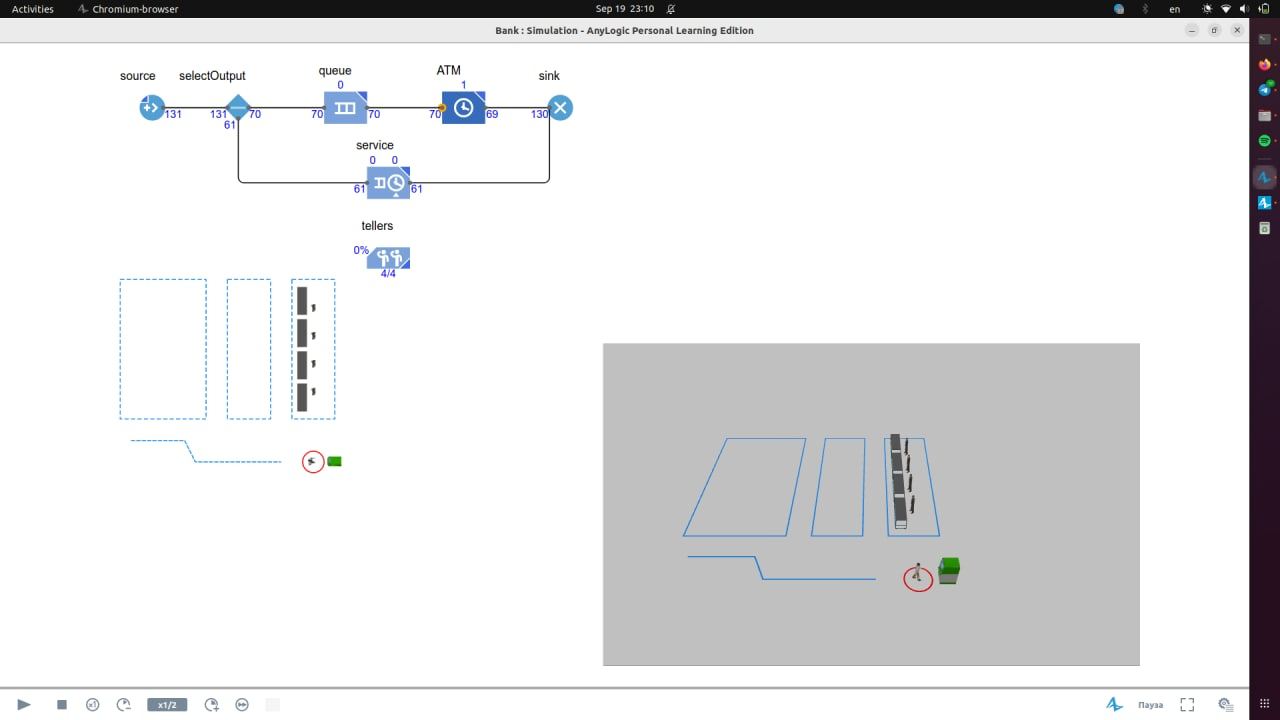
\includegraphics[scale=0.27]{anylogic_bank3}
	\caption{Усложнение модели СМО в среде AnyLogic}
	\label{fig:anylogic_bank3}
\end{figure}

\newpage

Также была добавлена анимация для новой части модели.\\

Добавим в модель сбор статистики. С помощью столбиковой диаграммы из палитры Статистика отобразим среднее время занятости банкомата и среднюю длину очереди:
\begin{figure}[h]
	\centering 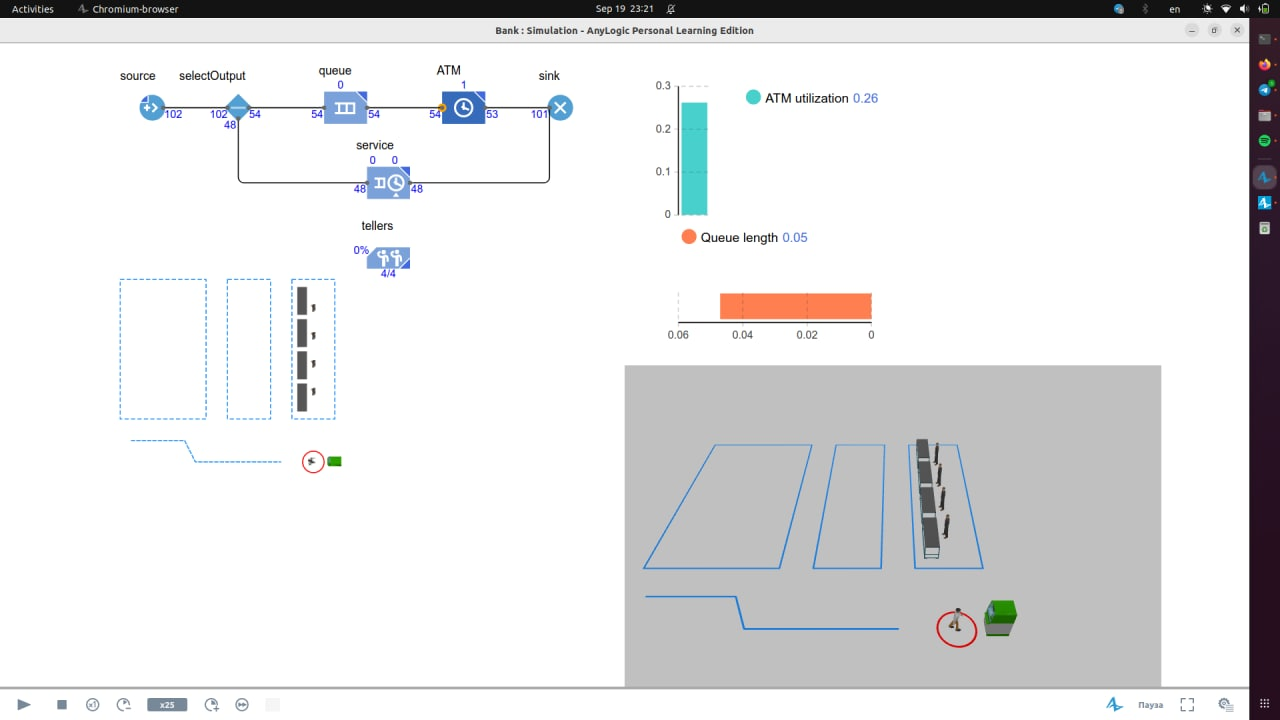
\includegraphics[scale=0.35]{anylogic_bank4}
	\caption{Добавление статистики среднего времени занятости банкомата и средней длины очереди}
	\label{fig:anylogic_bank4}
\end{figure}

С помощью гистограммы из палитры Статистика отобразим время ожидания и время обслуживания в системе.
\begin{figure}[h]
	\centering 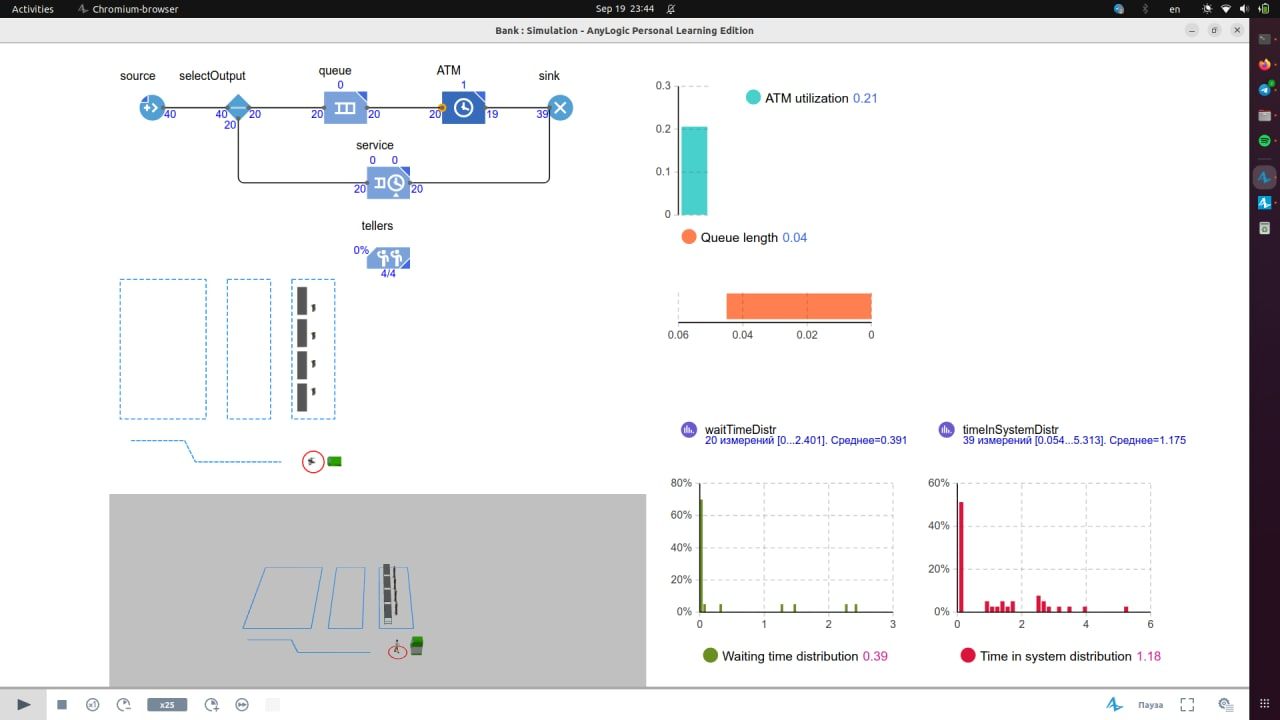
\includegraphics[scale=0.35]{anylogic_bank5}
	\caption{Добавление статистики времени ожидания и времени обслуживания в системе}
	\label{fig:anylogic_bank5}
\end{figure}

На гистограммах видно, что система работает хорошо, очереди маленькие, клиентов обслуживают быстро.